\documentclass[a4paper,11pt]{article}

\usepackage[francais]{babel} 
\usepackage[utf8]{inputenc}
\usepackage[cyr]{aeguill}
\usepackage{stmaryrd}

\usepackage{lmodern} %Type1-font for non-english texts and characters
\usepackage{caption}
\usepackage{subcaption}

\usepackage{graphicx}
\usepackage{hyperref}

\usepackage{epstopdf}


%\hypersetup{	
%colorlinks=true,   %colorise les liens 
%breaklinks=true,  %permet le retour à la ligne dans les liens trop longs 
%urlcolor= blue,    %couleur des hyperliens 
%linkcolor= black, %couleur des liens internes 
%citecolor=black,	 %couleur des références 
%pdftitle={Compte rendu \emph{HW1 Report}, %informations apparaissant dans 
%pdfauthor={Mélisande Zonta}, %les informations du document 
%pdfsubject={HW1 Report}	%sous Acrobat. 
%} 

%% Math Packages 
\usepackage{amsmath}
\usepackage{amsthm}
\usepackage{amsfonts}
\usepackage{amssymb}
\usepackage{mathrsfs}
\usepackage{pst-all}
\usepackage{lscape}
\usepackage{pdfpages}
\usepackage{mathabx}


\usepackage{color, colortbl}
\definecolor{lightgray}{gray}{0.85}
\usepackage{multirow}
\usepackage[Algorithme]{algorithm}
\usepackage[noend]{algpseudocode}
\usepackage{tikz}

%\renewcommand{\algorithmicdo}{\textbf{faire}}
%\renewcommand{\algorithmicwhile}{\textbf{tant que}}


\usepackage{a4wide} %%Smaller margins = more text per page.
\usepackage{fancyhdr} %%Fancy headings

\setcounter{secnumdepth}{5}
\setcounter{tocdepth}{5}


\DeclareMathOperator*{\argmax}{arg\,max}
\DeclareMathOperator*{\argmin}{arg\,min}
\graphicspath{{/Users/jacquelineroudes/Documents/GTL_courses/Data_Visual_Analytics}}

\begin{document}

%\pagestyle{fancy}

\begin{titlepage}
\vspace*{\stretch{1}}

\begin{center}

\includegraphics[scale=0.4]{GT_logo.jpeg}
\end{center}
\vspace*{\stretch{1}}
\hrulefill
\begin{center}\bfseries\huge
   HW1 Report \\
    R Programming\\
    \hrulefill
\end{center}
%\hfill
\vspace*{1cm}
\begin{minipage}[t]{0.3\textwidth}
  \begin{flushleft} \large
    \emph{Subject : }\\
    CSE6242 Spring 2017 - OMS}\\
  \end{flushleft}
\end{minipage}
\begin{minipage}[t]{0.6\textwidth}
  \begin{flushright} \large
    \emph{Authors :} \\
    Melisande Zonta \\
  \end{flushright}
\end{minipage}
\vspace*{\stretch{2}}
\begin{flushright}
       Le \today 
\end{flushright} 

\end{titlepage}


\section{Get Familiar with R}

 In addition of some syntax particularities, what strikes me most in the R programming language is the power of dataframes. 
 Indeed, at first sight, this object has rows and columns as a matrix, however the big difference stands in the possibility to store various types of objects (mode character, mode numeric, mode logical...).
 While this kind of storage can be seen in the list which is is a special vector with elements of different modes including lists themselves, the list's content is not represented as an array. 
The distinguishing feature between a dataframe and a list is the constraint in the first of having a similar length of elements which explains the organisation in columns. 
So let's take an example of a ranking between countries which is a particularly convenient for dataframe. Datas were extracted from this document : \url{http://www.clesdusocial.com/IMG/pdf/europe-sociale-chiffres-classements.pdf}.
To create our data-frame, we have to gather the elements of each category in a list and then call the R function data.frame().
\begin{figure}[H]
\centering
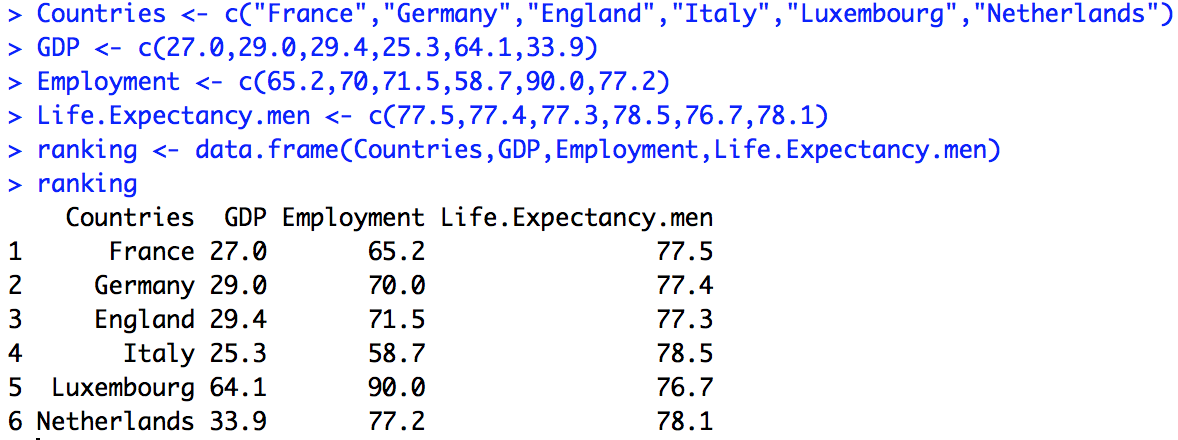
\includegraphics[width=.8\textwidth]{figure2}
 \caption{Creation of the first data-frame}
\label{figure2}
\end{figure}
We can build another one on the same pattern.
\begin{figure}[H]
\centering
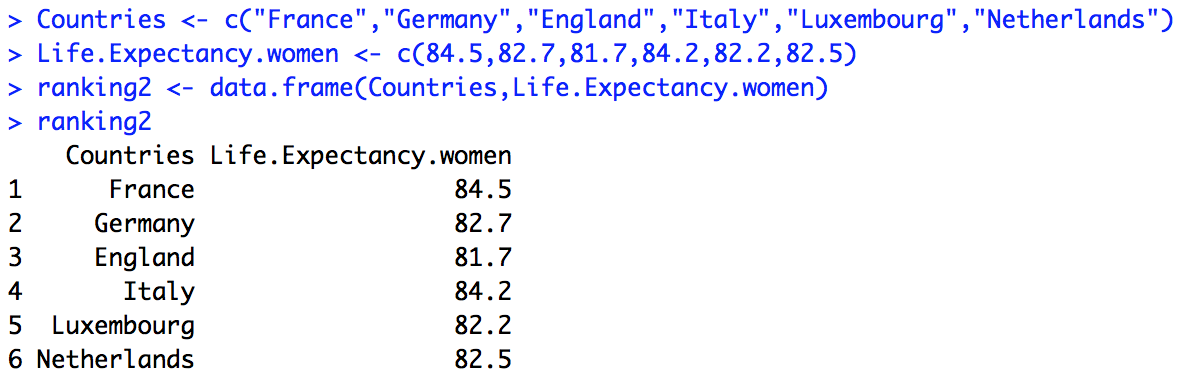
\includegraphics[width=.8\textwidth]{figure3}
 \caption{Creation of the second data-frame}
\label{figure3}
\end{figure}
One powerful function in R is the possibility of merging two data-frames.
\begin{figure}[H]
\centering
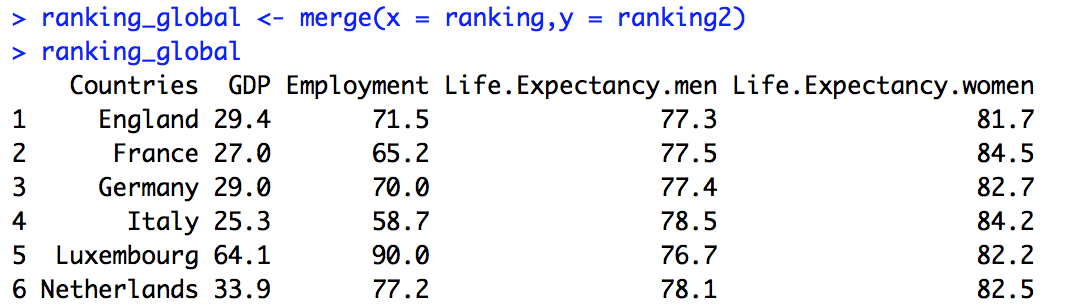
\includegraphics[width=.8\textwidth]{figure4}
 \caption{Merger of the two data-frames}
\label{figure4}
\end{figure}
We can visualize in our workspace the array.
\begin{figure}[H]
\centering
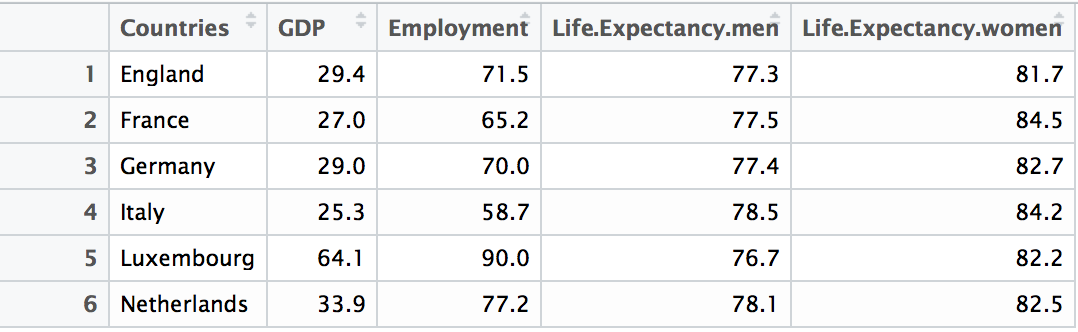
\includegraphics[width=.8\textwidth]{figure6}
 \caption{Storage of the global array}
\label{figure6}
\end{figure}
There are different ways of accessing the array's values.
\begin{figure}[H]
\centering
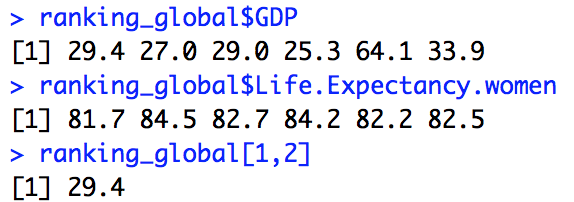
\includegraphics[width=.6\textwidth]{figure5}
 \caption{How to access to variables ?}
\label{figure5}
\end{figure}

 
\section{Compare Results to Built-in R Function}

\begin{figure}[H]
\centering
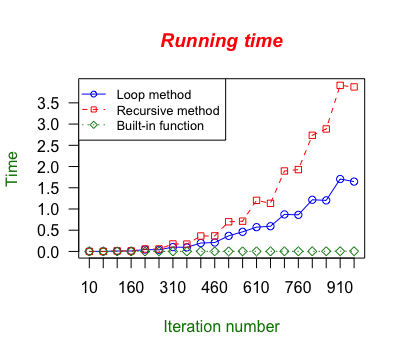
\includegraphics[width=.6\textwidth]{Time_100_iterations}
 \caption{Comparison between the 3 function over 1000 iterations}
\label{courbe1}
\end{figure}

\begin{figure}[H]
\centering
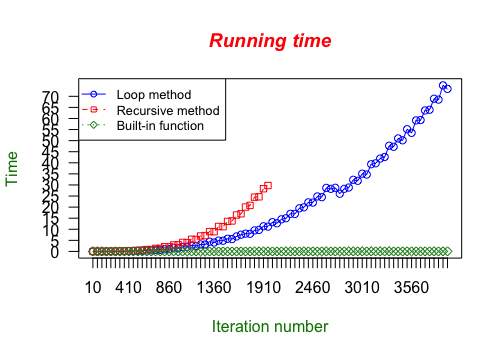
\includegraphics[width=.6\textwidth]{time_4000_iteration}
 \caption{Comparison between the 3 function over 4000 iterations}
\label{courbe2}
\end{figure}



\end{document}